\documentclass[a4paper, 11pt, oneside]{book}
\usepackage[a4paper, total={6.5in, 10in}]{geometry}
\usepackage{hyperref}

\usepackage[svgnames]{xcolor}
\usepackage{graphicx}
\usepackage[utf8]{inputenc}
\usepackage[T1]{fontenc}
\usepackage{PTSerif}
\usepackage{listings}
\usepackage{booktabs}
\usepackage{fouriernc}
\usepackage{makecell}
\usepackage{fontawesome}
\usepackage{hyperref}
\usepackage{tabularx}
\usepackage{xparse}
\usepackage{amssymb, amsmath}
\usepackage[many]{tcolorbox}
\tcbuselibrary{listings}

\newcommand{\cxoneflow}{\href{https://github.com/checkmarx-ts/cxone-flow}{\textbf{CxOneFlow}}\space}


\begin{document}

\begin{titlepage}
    \thispagestyle{empty}
    \centering
    
\includegraphics[scale=.4]{graphics/cx_logo-dark.png}
    \vfill
    \textcolor{Sienna}{\Huge CxOne-Flow\\DEV}
    \vfill
    {\Large\textbf{Nathan Leach, OSCP, CSSLP\\Checkmarx Principal Solution Architect}}
\end{titlepage}

\newpage


\tableofcontents


\newtcblisting{xml}[3]{
    listing only,
    title=<#1> #2 #3,
    width=\textwidth,
    listing options={
        basicstyle=\small\ttfamily,
        breaklines=true,
        columns=fullflexible,
    },
}

\newtcblisting{code}[3]{
    listing only,
    title=#1 #2 #3,
    width=\textwidth,
    listing options={
        basicstyle=\small\ttfamily,
        breaklines=true,
        columns=fullflexible,
    },
}


\part{Operation}
\chapter{Overview}\label{sec:overview}

\section{Workflow Overview}

\cxoneflow has origins in CxFlow for the CxSAST product, which is the predecessor to \cxone.  CxFlow
had a variety of functions and deployment options related to orchestrating scans in CxSAST and sending
result feedback to issue trackers.  \cxoneflow will also orchestrate scans but is adapted to the
concepts of \cxone.

The \cxoneflow logic for how scans are orchestrated is very similar to that of CxFlow.  The basic
logic flow is that scans are executed when:

\begin{itemize}
    \item If a Push is made to a repository's protected branch, that protected branch is scanned.
    \item If a Pull Request is opened that targets a protected branch, a scan is performed on
    the source branch.
    \item If a Push is made to a branch that is the source of an open Pull Request that targets
    a protected branch, that branch is scanned.
\end{itemize}


\cxoneflow follows this workflow logic upon the receipt of a webhook event payload generated by the SCM.
The code from the repository to be scanned is cloned by \cxoneflow, collected into a zip file, then submitted
for a scan to \cxone.  When the scan is submitted, the cloned code is deleted.


\section{Deployment Overview}

The method of deployment for \cxoneflow is intended to integrate scanning of all enterprise repositories
with a minimal amount of configuration.  The best method for deployment is to configure source control web
hooks where they will emit events for the largest possible number of repositories.  In many source control
systems, this can be done at a global or organization level.  The web hooks will be configured to send events
to a \cxoneflow endpoint specific to the type of source control system.

Figure \ref{fig:cxoneflow-deployment} is a \cxoneflow deployment diagram. The key points of the diagram:

\begin{itemize}
    \item A single instance or clustered install of \cxoneflow can be used as the endpoint for multiple
    SCM instances.
    \item There may be more than one instance of an SCM type.
    \item Each SCM instance may have one or more logical groups of repositories.  For example:
    \begin{itemize}
        \item Azure DevOps has \textbf{Collections} and each collection has a \textbf{Project} where
        each project will contain repositories.
        \item GitHub has \textbf{Organizations} where each organization will contain repositories.
        \item BitBucket Data Center has \textbf{Projects} where each project will contain repositories.
    \end{itemize}
    \item There may be multiple \cxone tenants where scans are to be invoked from an SCM or SCM
    logical group of repositories.
\end{itemize}

The \cxoneflow configuration allows each endpoint to be configured such that it orchestrates
scans in the correct \cxone instance and tenant for the SCM that emits the web hook event.
\cxoneflow is compatible with Checkmax One hosted single-tenant, hosted multi-tenant, and self-hosted
instances.

\begin{figure}[ht]
    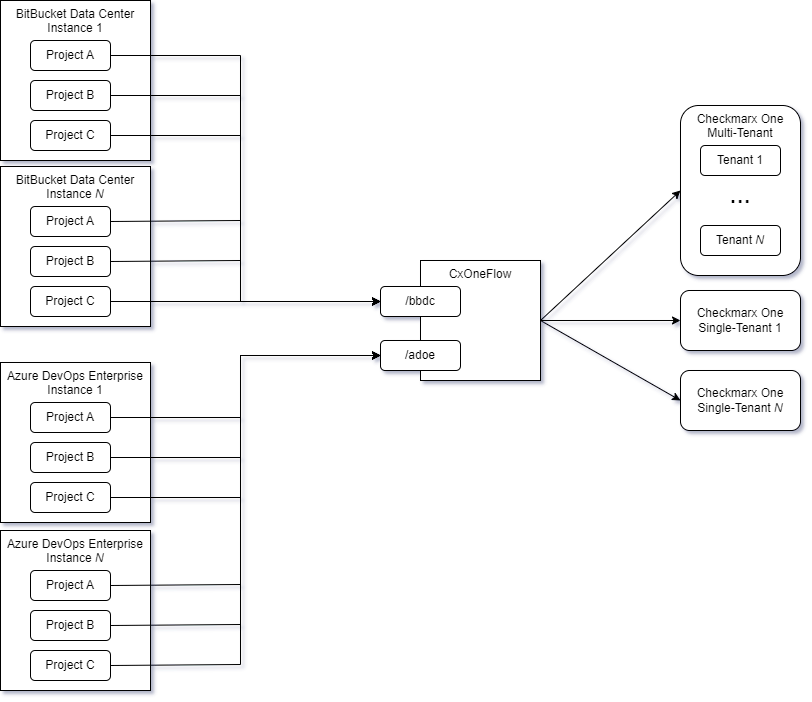
\includegraphics[width=\textwidth]{graphics/cxoneflow-deployment.png}
    \caption{\cxoneflow Deployment Diagram}
    \label{fig:cxoneflow-deployment}
\end{figure}


\chapter{Quickstart}

To get up and running with a basic configuration of \cxoneflow, these are the following steps:


\section{Step 1: Create a basic configuration YAML file}

The full configuration documentation can be found in Section \ref{sec:op-config}. To fully configure the \cxoneflow you'll need
the following information that will be used when composing the configuration YAML file:

\begin{itemize}
    \item A \cxone API Key or OAuth client id + client secret.
    \item Credentials appropriate for communicating with the Git server's API.
    \item Credentials used to clone Git repositories if the clone credentials must be different than the credentials used for API access.
\end{itemize}

\noindent\\The types of credentials may vary based on how the SCM server is configured or how \cxoneflow
integrates with the SCM.

\section{Step 2: Execute the \cxoneflow Container}

The published \cxoneflow container can be executed with the proper runtime configuration.  Please refer
to Section \ref{sec:runtime-config} for instructions about starting the \cxoneflow container instance with
the proper runtime configuration. Section \ref{sec:deployment} has additional deployment information that
may be useful in choosing how and where to host the \cxoneflow instance.


\section{Step 3: Configure SCM Webhooks}

Please refer to the chapter for your SCM platform in Part \ref{part:scms} for details about webhook configuration.



\chapter{Configuration}


\section{Runtime Configuration}\label{sec:runtime-config}

\subsection{SSL}

\subsubsection{Trusting Self-Signed Certificates}\label{sec:self-signed-certs}

While the CheckmarxOne system uses TLS certificates signed by a public CA, it is possible that
corporate proxies use certificates signed by a private CA. If so, it is possible to
import custom CA certificates when using \cxoneflow.

\noindent\\The custom certificates must meet the following criteria:

\begin{itemize}
    \item Must be in the PEM format.
    \item Must be in a file ending with the extension .crt.
    \item Only one certificate is in the file.
    \item Must be mapped to the container path /usr/local/share/ca-certificates.
\end{itemize}


\noindent\\As an example, if using Docker, it is possible to map a local file to a file in the container with this mapping option added to the container execution command line:

\begin{code}{Custom CA Mapping Option}{[Docker]}{}
-v $(pwd)/custom-ca.pem:/usr/local/share/ca-certificates/custom-ca.crt
\end{code}

\subsubsection{Configuring SSL for the \cxoneflow Endpoint}

To make the \cxoneflow endpoint use SSL for communication, obtain an SSL certificate public/private key pair
and then set the following environment variables in the runtime environment:

\begin{table}[h]
    \caption{SSL Environment Variables}        
    \begin{tabularx}{\textwidth}{ll}
        \toprule
        \textbf{Variable} & \textbf{Description}\\
        \midrule
        \texttt{SSL\_CERT\_PATH} & \makecell[l]{The path to the server's SSL certificate in PEM format.}\\
        \midrule
        \texttt{SSL\_CERT\_KEY\_PATH} & \makecell[l]{The path to the certificate's unencrypted private key.}\\
        \bottomrule
    \end{tabularx}
\end{table}

\noindent\\If your SSL certificate is self-signed or signed with a non-public CA, you'll want
to import the custom CA as described in Section \ref{sec:self-signed-certs}.


\subsection{Rutime Control Environment Variables}

\begin{table}[h]
    \caption{Runtime Control Environment Variables}        
    \begin{tabularx}{\textwidth}{lccl}
        \toprule
        \textbf{Variable} & \textbf{Required} & \textbf{Default} & \textbf{Description}\\
        \midrule
        \texttt{CXONEFLOW\_WORKERS} & No & \texttt{(\# of CPUs / 2)} & \makecell[l]{The number of worker processes\\used for parallel execution. The\\maximum value will be\\set at \texttt{(\# of CPUs - 1)}}\\
        \midrule
        \texttt{LOG\_LEVEL} & No & \texttt{INFO} & \makecell[l]{The logging verbosity level.  Set to\\\texttt{DEBUG} for increased logging\\verbosity.}\\
        \midrule
        \texttt{CONFIG\_YAML\_PATH} & No & \texttt{/opt/cxone/config.yaml} & \makecell[l]{The path to the configuration\\YAML file.}\\
        \midrule
        \texttt{CXONEFLOW\_HOSTNAME} & No & \texttt{localhost} & \makecell[l]{The virtual hostname of the\\\cxoneflow endpoint.}\\
        \bottomrule
    \end{tabularx}
\end{table}


\newpage

\section{Operational Configuration}\label{sec:op-config}

The operational configuration is done using a YAML file mapped at \texttt{/opt/cxone/config.yaml}
by default.  

\subsection{YAML Configuration Examples}

\subsubsection{Basic YAML Configurations}

The following example shows a minimal \cxoneflow configuration that defines the following:

\begin{enumerate}
    \item Files containing secrets are located at \texttt{/run/secrets}.
    \item One BitBucket Data Center SCM connection configuration to handle all webhook payloads
    POSTed to the \texttt{/bbdc} endpoint.
    \item One catch-all route for clone-urls using the regular expression \texttt{.*}
    \item The SCM's base URL located at \texttt{https://scm.corp.com}
    \item The shared secret used to validate webhook payloads located in the file \texttt{/run/secrets/scm-shared-secret}
    \item The API and clone authorization using a PAT in a file located at \texttt{/run/secrets/scm-token-secret}
    \item The CheckmarxOne tenant name of \texttt{mytenant}
    \item The CheckmarxOne API credentials using an \texttt{oauth} client with:
    \begin{enumerate}
        \item The client identifier located in the file \texttt{/run/secrets/my-oauth-id}
        \item The client secret located in the file \texttt{/run/secrets/my-oauth-secret}
    \end{enumerate}
    \item Using the CheckmarxOne multi-tenant US region IAM endpoint.
    \item Using the CheckmarxOne multi-tenant US region API endpoint.
\end{enumerate}

\begin{code}{Minimal YAML Configuration Example \#1}{[CxOne: oauth]}{[SCM: token auth]}
secret-root-path: /run/secrets

bbdc:
    - service-name: BitBucket DC
      repo-match: .*
      connection:
        base-url: https://scm.corp.com
        shared-secret: scm-shared-secret
        api-auth:
            token: scm-token-secret
      cxone:
        tenant: mytenant
        oauth:
            client-id: my-oauth-id
            client-secret: my-oauth-secret
        iam-endpoint: US
        api-endpoint: US
\end{code}

\pagebreak
\noindent\\An alternate minimal example using different authorization options:

\begin{code}{Minimal YAML Configuration Example \#2}{[CxOne: api-key]}{[SCM: basic/ssh auth]}
secret-root-path: /run/secrets

bbdc:
    - service-name: BitBucket DC
      repo-match: .*
      connection:
      base-url: https://scm.corp.com
      shared-secret: scm-shared-secret
      api-auth:
          username: scm-username-secret
          password: scm-password-secret
      clone-auth:
          ssh: scm-ssh-key-secret
      cxone:
        tenant: mytenant
        api-key: my-cxone-api-key
        iam-endpoint: US
        api-endpoint: US
\end{code}
    
\pagebreak
\noindent\\An alternate minimal example using for an Azure DevOps Enterprise
SCM:

\begin{code}{Minimal YAML Configuration Example \#2}{[CxOne: api-key]}{[SCM: basic/ssh auth]}
secret-root-path: /run/secrets

adoe:
    - service-name: MyADO
      repo-match: .*
      connection:
      base-url: https://scm.corp.com
      shared-secret: scm-shared-secret
      api-auth:
          username: scm-username-secret
          password: scm-password-secret
      clone-auth:
          ssh: scm-ssh-key-secret
      cxone:
        tenant: mytenant
        api-key: my-cxone-api-key
        iam-endpoint: US
        api-endpoint: US
\end{code}


\newpage
\noindent\\This example shows a \cxoneflow configuration explicitly setting default options in a service 
configuration for a single SCM.  The minimal examples leave several of these options as default.

The \texttt{scan-config} element has been added to this configuration to
demonstrate some of the controls that can be implemented over scan options.  In this
example, static Project and Scan tags are defined.  Also defined is the selection
of engines for the scan with some options defined as supported by the engine.
Documentation for the option keys can be found in the Checkmarx
\extlink{https://checkmarx.stoplight.io/docs/checkmarx-one-api-reference-guide/branches/main/f601dd9456e80-run-a-scan}{Scan REST API}
documentation and have the descriptions documented in the
\extlink{https://docs.checkmarx.com/en/34965-324311-settings-for-specific-scanners.html}{Scanners Settings}
documentation.

While there are options to apply scan configurations via \texttt{scan-config} elements, it is often the case that defining the scan configuration
in \cxoneflow will have undesirable results.  When defined in the \cxoneflow configuration, the configuration will explicitly override \cxone
tenant and project level default scan configurations.  Details about utilizing the \cxone configuration options for best results with \cxoneflow
can be found in Section \ref{sec:deployment-scan-defaults}.

\begin{code}{Full YAML Configuration Example}{[CxOne: oauth]}{[SCM: token auth]}
secret-root-path: /run/secrets
server-base-url: https://cxoneflow.mydomain.com:8443/

bbdc:
    - service-name: BitBucket DC
      repo-match: .*
      scan-config:
          default-scan-engines:
              sca:
                  exploitablePath: "True"
              sast:
                  presetName: ASA Premium
                  incremental: "False"
                  fastScanMode: "True"
                  filter: "!**/node_modules,!**/test*"
                  languageMode: multi
              kics:
              apisec:
          default-scan-tags:
              scan-service: BitBucket DC
          default-project-tags:
              onboarded-by: CxOneFlow
      connection:
          base-url: https://scm.corp.com
          shared-secret: scm-shared-secret
          timeout-seconds: 60
          retries: 3
          proxies:
            http: http://proxy.corp.com:8080
            https: http://proxy.corp.com:8080
          api-auth:
              token: scm-token-secret
      cxone:
          tenant: mytenant
          oauth:
              client-id: my-oauth-id
              client-secret: my-oauth-secret
          iam-endpoint: US
          api-endpoint: US
          timeout-seconds: 60
          retries: 3
          proxies:
            http: http://proxy.corp.com:8080
            https: http://proxy.corp.com:8080
\end{code}


\pagebreak
The next example shows a configuration where \cxoneflow has endpoint handlers for both
BitBucket Data Center and Azure DevOps Enterprise.  Each SCM is configured to handle multiple distinct
projects to demonstrate the use of multiple authentication methods.  All the SCM endpoints
orchestrate scans in a single \cxone tenant.

\begin{code}{Multi-SCM/Multi-Org YAML Configuration Example}{}{}
secret-root-path: /run/secrets
server-base-url: https://cxoneflow.mydomain.com:8443/
adoe-connection: &adoe-con
    base-url: http://adoe.scm.org/
    shared-secret: scm-shared-secret
bbdc-connection: &bbdc-con
    base-url: http://bbdc.scm.org
    shared-secret: scm-shared-secret
adoe:
    - service-name: ADO-EastCoast
        repo-match: .*East
        connection:
        <<: *adoe-con
        api-auth: 
            token: adoe-token-secret
        clone-auth: &clone-ssh
            ssh: ssh-priv-key
        cxone: &cxone
        tenant: my_tenant
        oauth:
            client-id: prod_client_id
            client-secret: prod_client_secret
        iam-endpoint: US
        api-endpoint: US
    - service-name: ADO-WestCoast
        repo-match: .*West
        connection:
        <<: *adoe-con
        api-auth:
            token: adoe-token-secret
        cxone: *cxone
bbdc:
    - service-name: BBDC-EastCoast
        repo-match: .*EAS
        connection:
        <<: *bbdc-con
        api-auth: 
            token: bbdc-token
        clone-auth: *clone-ssh
        cxone: *cxone
    - service-name: BBDC-WestCoast
        repo-match: .*WES
        connection:
        <<: *bbdc-con
        api-auth:
            token: bbdc-token
        cxone: *cxone
\end{code}



\subsubsection{Complex YAML Configurations using YAML Anchors}

For complex configurations, it is possible to use 
\href{https://docs.docker.com/compose/compose-file/10-fragments/}{YAML Anchors}
to avoid repeating some section definitions.  When using YAML anchors, it may be useful
to use a \href{https://onlineyamltools.com/convert-yaml-to-json}{YAML-to-JSON} conversion tool that shows the JSON generated from the YAML
definition

\noindent\\This example demonstrates defining common connection parameters that can be applied
to all connection definitions:


\begin{code}{Compacted Full YAML Configuration Example}{[CxOne: oauth]}{[SCM: token auth]}
secret-root-path: /run/secrets

my-connection-params: &common-connection-params
    timeout-seconds: 60
    retries: 3
    ssl-verify: True
    proxies:
    http: http://proxy.corp.com:8080
    https: http://proxy.corp.com:8080


bbdc:
    - service-name: BitBucket DC
      repo-match: .*
      scan-config:
          default-scan-engines:
              sca:
                  exploitablePath: "True"
              sast:
                  presetName: ASA Premium
                  incremental: "False"
                  fastScanMode: "True"
                  filter: "!**/node_modules,!**/test*"
                  languageMode: multi
              kics:
              apisec:
          default-scan-tags:
              scan-service: BitBucket DC
          default-project-tags:
              onboarded-by: CxOneFlow
      connection:
          base-url: https://scm.corp.com
          shared-secret: scm-shared-secret
          api-auth:
              token: scm-token-secret
          <<: *common-connection-params
      cxone:
          tenant: mytenant
          oauth:
              client-id: my-oauth-id
              client-secret: my-oauth-secret
          iam-endpoint: US
          api-endpoint: US
          <<: *common-connection-params
\end{code}


\noindent\\It is common to see a scenario where there are multiple organizations
using the same SCM instance.  A single \cxoneflow instance can be configured to accept
webhook events from all repos in each organization by using the \texttt{repo-match}
regular expression.  When a webhook payload is received, the \texttt{repo-match}
regular expression is applied to the clone URI until a match is found.

\noindent\\The example YAML below is used to demonstrate how \cxoneflow could be configured
for mulitple organizations in a single SCM. In the example, YAML anchors are utilized to 
re-use the common settings for each SCM organization.  Each organization, in this case, 
exists in the same SCM server and shares the same Checkmarx One instance.

\begin{code}{SCM Multi-Org YAML Configuration Example}{[CxOne: oauth]}{[SCM: token auth]}
secret-root-path: /run/secrets

my-connection-params: &common-connection-params
    timeout-seconds: 60
    retries: 3
    ssl-verify: True
    proxies:
    http: http://proxy.corp.com:8080
    https: http://proxy.corp.com:8080

bbdc:
    - service-name: BBDC-West
      repo-match: .*west
      scan-config: 
          default-scan-engines: &common-engine-config
              sca:
                  exploitablePath: "True"
              sast:
                  presetName: ASA Premium
                  incremental: "False"
                  fastScanMode: "True"
                  filter: "!**/node_modules,!**/test*"
                  languageMode: multi
              kics:
              apisec:
          default-scan-tags:
              scan-service: BBDC-West
          default-project-tags:
              onboarded-by: CxOneFlow
              region: West
      connection:
          base-url: https://scm.corp.com
          shared-secret: scm-west-org-shared-secret
          api-auth:
              token: scm-token-secret
          <<: *common-connection-params
      cxone: &cxone-config
          tenant: mytenant
          oauth:
              client-id: my-oauth-id
              client-secret: my-oauth-secret
          iam-endpoint: US
          api-endpoint: US
          <<: *common-connection-params
    - service-name: BBDC-East
      repo-match: .*east
      scan-config: 
          default-scan-engines: *common-engine-config
          default-scan-tags:
              scan-service: BBDC-East
          default-project-tags:
              onboarded-by: CxOneFlow
              region: East
      connection:
          base-url: https://scm.corp.com
          shared-secret: scm-east-org-shared-secret
          api-auth:
              token: scm-token-secret
          <<: *common-connection-params
      cxone: *cxone-config
\end{code}



\subsection{YAML Configuration Elements}

\subsubsection{YAML Root}\label{sec:yaml-root}

The root of the YAML configuration will contain the \texttt{secret-root-path} element
and one or more unique SCM configuration monikers.  The following SCM configuration monikers
are currently supported:

\begin{itemize}
    \item \texttt{bbdc} for BitBucket Data Center hook payloads targetting the \texttt{/bbdc}
    webhook payload receiver endpoint.
\end{itemize}


\noindent\\The value for \texttt{secret-root-path} is the path to a directory that contains one
or more files containing secret values.  The names to these files are referenced elsewhere
in the YAML configuration file as described in
\hyperref[sec:scm-block-element]{YAML SCM Configuration Element}.


\subsubsection{YAML SCM Configuration Element}\label{sec:scm-block-element}

The SCM configuration element is the same for all SCM monikers. The element is a list with
one or more entries corresponding to a clone URL regular expression match.  The entry
that first matches the clone URL received in the webhook payload is used to configure
the workflow execution parameters.  Table \ref{tab:scm-section-keys} explains the SCM
configuration keys for each SCM configuration list entry.

\begin{table}[h]
    \caption{SCM Configuration YAML Element}  
    \label{tab:scm-section-keys}      
    \begin{tabularx}{\textwidth}{lcl}
        \toprule
        \textbf{Key} & \textbf{Required} & \textbf{Description}\\
        \midrule
        \texttt{service-name} & Yes & \makecell[l]{A moniker for the route match that is used for logging purposes.}\\
        \midrule
        \texttt{repo-match} & Yes & \makecell[l]{A regex applied to the source repository.  If the webhook payload has\\a clone URL that matches the regex, this configuration is used to\\orchestrate the scanning.}\\
        \midrule
        \texttt{scan-config} & No & \makecell[l]{Elements that define the default scan configuration.  This element\\is described in the section\\"\hyperref[sec:scan-config-element]{YAML Configuration Element: \texttt{scan-config}}"}\\
        \midrule
        \texttt{connection} & Yes & \makecell[l]{SCM connection parameters. This element\\is described in the section\\"\hyperref[sec:connection-element]{YAML Configuration Element: \texttt{connection}}"}\\
        \midrule
        \texttt{cxone} & Yes & \makecell[l]{The connection configuration for the CheckmarxOne API. This\\element is described in the section\\"\hyperref[sec:cxone-element]{YAML Configuration Element: \texttt{cxone}}"}\\
        \bottomrule
    \end{tabularx}
\end{table}


\paragraph{YAML Configuration Element: \texttt{scan-config} }\label{sec:scan-config-element}

\noindent\\\\The \texttt{scan-config} element, described in Table \ref{tab:scan-config-section-keys}, allows for default configurations to be applied to each scan.

\begin{table}[h]
    \caption{\texttt{scan-config} YAML Element}  
    \label{tab:scan-config-section-keys}      
    \begin{tabularx}{\textwidth}{lcl}
        \toprule
        \textbf{Key} & \textbf{Required} & \textbf{Description}\\
        \midrule
        \texttt{default-scan-engines} & No & \makecell[l]{A element that follows the format\\\texttt{<engine-name>:<engine config option dictionary>}\\corresponding to the configuration element of the\\\href{https://checkmarx.stoplight.io/docs/checkmarx-one-api-reference-guide/branches/main/f601dd9456e80-run-a-scan}{Checkmarx One scan API}.}\\
        \midrule
        \texttt{default-scan-tags} & No &  \makecell[l]{A dictionary of static key:value pairs that are assigned to\\each scan.}\\
        \midrule
        \texttt{default-project-tags} & No & \makecell[l]{A dictionary of static key:value pairs that are assigned\\to each project upon project creation.}\\
        \bottomrule
    \end{tabularx}
\end{table}


\paragraph{YAML Configuration Element: \texttt{cxone} }\label{sec:cxone-element}

\noindent\\\\The \texttt{cxone} element, described in Table \ref{tab:cxone-section-keys}, 
describes the CheckmarxOne API connection parameters.


\begin{table}[h]
    \caption{\texttt{cxone} YAML Element}  
    \label{tab:cxone-section-keys}      
    \begin{tabularx}{\textwidth}{lccl}
        \toprule
        \textbf{Key} & \textbf{Required} & \textbf{Default} & \textbf{Description}\\
        \midrule
        \texttt{tenant} & Yes & N/A & \makecell[l]{The name of the CheckmarxOne tenant.}\\
        \midrule
        \texttt{iam-endpoint} & Yes & N/A & \makecell[l]{This can be a fully qualified domain name of a server\\or a multi-tenant IAM endpoint moniker as described\\in Appendix \ref{sec:endpoint-monikers}.}\\
        \midrule
        \texttt{api-endpoint} & Yes & N/A & \makecell[l]{This can be a fully qualified domain name of a server\\or a multi-tenant API endpoint moniker as described\\in Appendix \ref{sec:endpoint-monikers}.}\\
        \midrule
        \texttt{timeout-seconds} & No & 60s & \makecell[l]{The number of seconds before a request for API\\results times out.}\\
        \midrule
        \texttt{retries} & No & 3 & \makecell[l]{The number of retries when the request fails.}\\
        \midrule
        \texttt{ssl-verify} & No & True & \makecell[l]{If False, server SSL certificates are not validated.}\\
        \midrule
        \texttt{proxies} & No & N/A & \makecell[l]{A dictionary of \texttt{<scheme>:<url>} pairs to use a proxy\\server for requests. See: \href{https://requests.readthedocs.io/en/latest/user/advanced/\#proxies}{Python "requests" proxies}.}\\
        \midrule
        \texttt{api-key} & No & N/A & \makecell[l]{If not defined, the \texttt{oauth} element must be defined.\\The value specifies a file name found under the path\\defined by \texttt{secret-root-path}.}\\
        \midrule
        \texttt{oauth} & No & N/A & \makecell[l]{If not defined, the \texttt{api-key} element must be defined.\\This contains two required elements \texttt{client-id}\\and \texttt{client-secret} where each value corresponds to\\a file name found under the path defined by\\\texttt{secret-root-path}. }\\
        \bottomrule
    \end{tabularx}
\end{table}


\pagebreak
\paragraph{YAML Configuration Element: \texttt{connection} }\label{sec:connection-element}

\noindent\\\\The \texttt{connection} element, described in Table \ref{tab:connection-section-keys}, 
describes the SCM connection parameters used for API access and cloning.


\begin{table}[h]
    \caption{\texttt{connection} YAML Element}  
    \label{tab:connection-section-keys}      
    \begin{tabularx}{\textwidth}{lccl}
        \toprule
        \textbf{Key} & \textbf{Required} & \textbf{Default} & \textbf{Description}\\
        \midrule
        \texttt{base-url} & Yes & N/A & \makecell[l]{The base url of the SCM server.}\\
        \midrule
        \texttt{shared-secret} & Yes & N/A & \makecell[l]{The shared secret configured in the SCM used to sign\\webhook payloads. The shared secret must meet the\\following minimum criteria: 20 characters long,\\contains at least 3 numbers, contains at least\\3 upper-case letters, and contains at least 2 special\\characters.}\\
        \midrule
        \texttt{timeout-seconds} & No & 60s & \makecell[l]{The number of seconds before a request for API\\results times out.}\\
        \midrule
        \texttt{retries} & No & 3 & \makecell[l]{The number of retries when the request fails.}\\
        \midrule
        \texttt{ssl-verify} & No & True & \makecell[l]{If False, server SSL certificates are not validated.}\\
        \midrule
        \texttt{proxies} & No & N/A & \makecell[l]{A dictionary of \texttt{<scheme>:<url>} pairs to use a proxy\\server for requests. See: \href{https://requests.readthedocs.io/en/latest/user/advanced/\#proxies}{Python "requests" proxies}.}\\
        \midrule
        \texttt{api-auth} & Yes & N/A & \makecell[l]{A dictionary of SCM authorization options\\for using the API.\\See: \hyperref[sec:api-auth-element]{YAML Configuration Element: \texttt{api-auth}}}\\
        \midrule
        \texttt{clone-auth} & No & \makecell[l]{\texttt{api-auth}} & \makecell[l]{Authorization options for performing clones when it\\differs from authorization for API requests.\\See: \hyperref[sec:clone-auth-element]{YAML Configuration Element: \texttt{clone-auth}}}\\
        \bottomrule
    \end{tabularx}
\end{table}

\pagebreak
\paragraph{YAML Configuration Element: \texttt{clone-auth} }\label{sec:clone-auth-element}

\noindent\\\\The \texttt{clone-auth} element is optional;  if not provided, the connection information defined
in \texttt{api-auth} will be used.  This element can contain the following key:value pair combinations:

\noindent\\\textbf{Token Authorization Elements}

\noindent\\To clone with a token, the following elements can appear under the \texttt{clone-auth}
element exclusive of other elements:

\begin{itemize}
    \item \texttt{token} - The value specifies a file name found under the path defined
    by \texttt{secret-root-path} containing a Personal Access Token (PAT).  This is required for
    token authorization.
    \item \texttt{username} - The value specifies a file name found under the path defined
    by \texttt{secret-root-path} containing a username associated with the PAT.  This is 
    optional; if not supplied, the default username of \texttt{git} is used.
\end{itemize}

\noindent\\\textbf{Basic Authorization Elements}

\noindent\\To clone with basic authorization, the following required elements can appear under the
\texttt{clone-auth} element exclusive of other elements:

\begin{itemize}
    \item \texttt{username} - The value specifies a file name found under the path defined
    by \texttt{secret-root-path} containing the username associated with the account used
    for authorization. 
    \item \texttt{password} - The value specifies a file name found under the path defined
    by \texttt{secret-root-path} containing the password associated with the account used
    for authorization. 
\end{itemize}

\noindent\\\textbf{SSH Authorization Elements}

\noindent\\To clone with SSH, the following required element can appear under the
\texttt{clone-auth} element exclusive of other elements:

\begin{itemize}
    \item \texttt{ssh} - The value specifies a file name found under the path defined
    by \texttt{secret-root-path} containing an unencrypted private SSH key.
\end{itemize}

\paragraph{YAML Configuration Element: \texttt{api-auth} }\label{sec:api-auth-element}

\noindent\\\\The \texttt{api-auth} element is required.  The authorization methods for \texttt{api-auth} 
are used to communicate with the SCM's API and can often be used for cloning repositories.  The
main difference between \texttt{api-auth} and \texttt{clone-auth} is that API access generally
does not support SSH authorization. If there is a need to clone using SSH, configure the SSH
authorization under the \texttt{clone-auth} element.  This element can contain the following
key:value pair combinations:

\noindent\\\textbf{Token Authorization Elements}

\noindent\\To access the SCM API or clone with a token, the following elements can appear under the 
\texttt{api-auth} element exclusive of other elements:

\begin{itemize}
    \item \texttt{token} - The value specifies a file name found under the path defined
    by \texttt{secret-root-path} containing a Personal Access Token (PAT).  This is required for
    token authorization.
    \item \texttt{username} - The value specifies a file name found under the path defined
    by \texttt{secret-root-path} containing a username associated with the PAT.  This is 
    optional and only used during cloning; if not supplied, the default username of \texttt{git} is used.
\end{itemize}

\noindent\\\textbf{Basic Authorization Elements}

\noindent\\To access the SCM API or clone with basic authorization, the following required elements can
appear under the \texttt{api-auth} element exclusive of other elements:

\begin{itemize}
    \item \texttt{username} - The value specifies a file name found under the path defined
    by \texttt{secret-root-path} containing the username associated with the account used
    for authorization. 
    \item \texttt{password} - The value specifies a file name found under the path defined
    by \texttt{secret-root-path} containing the password associated with the account used
    for authorization. 
\end{itemize}






\part{Source Control Managers}\label{part:scms}
\chapter{BitBucket Data Center}

\section{About BitBucket Data Center}

BitBucket Data Center is often confused with BitBucket Cloud; it should be noted that
the \cxoneflow configuration for BitBucket Data Center is not compatible with BitBucket Cloud.

\noindent\\The \cxoneflow endpoint \texttt{/bbdc} is the handler for all webhook event
payloads originating from BitBucket Data Center.  


\section{Webhook Configuration}

BitBucket Data Center can assign web hooks at the Project (aka Organization) level as well as at the
repository level.  Deploying web hook configurations for an enterprise-scale SCM is generally better
at the organization level since it will apply to all repositories in the organization.  Deploying
at the repository level is mostly suitable for testing purposes only.

Figure \ref{fig:bbdc-project-config} shows the BitBucket Data Center project configuration screen.  The
project key will appear in clone URLs and can be used as part of the regular expression 
placed in the \texttt{repo-match} configuration element.  Please see Section \ref{sec:scm-block-element} 
for a description of the \texttt{repo-match} configuration element.

The project's "Webhooks" configuration can be used to configure the \cxoneflow endpoint 
\texttt{/bbdc} to receive webhook events for each repository in the organization.  

\begin{figure}[h]
    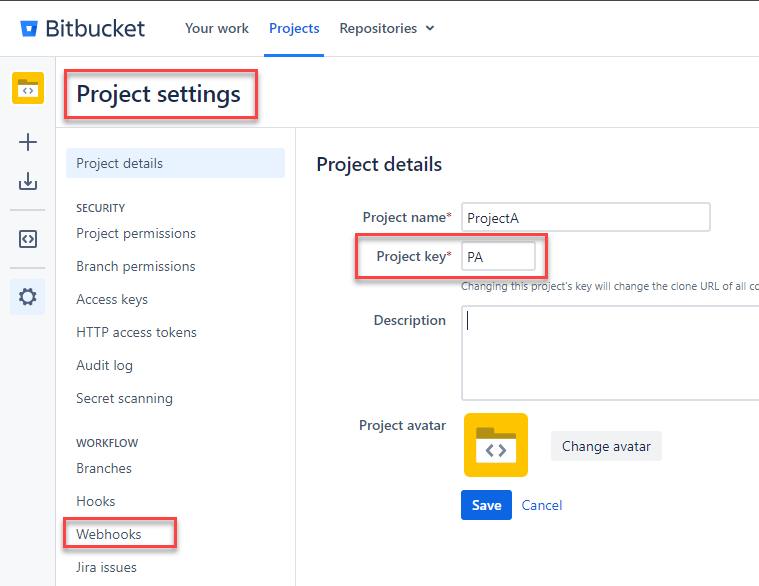
\includegraphics[width=\textwidth]{graphics/bbdc-project-config.png}
    \caption{BitBucket Data Center Project Configuration}
    \label{fig:bbdc-project-config}
\end{figure}

\begin{figure}[h]
    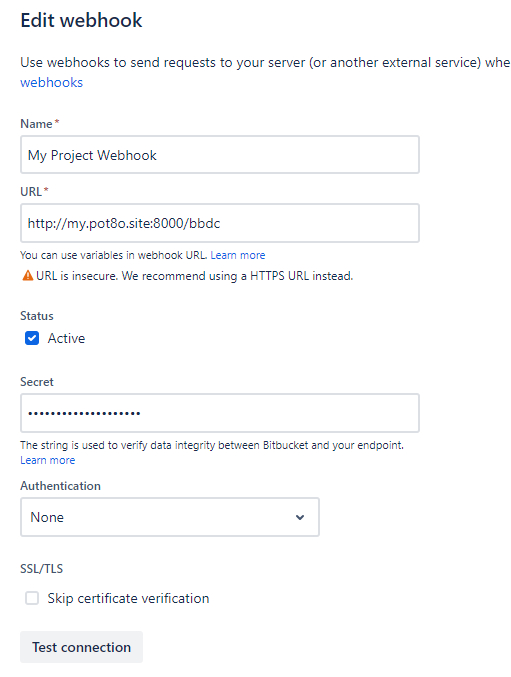
\includegraphics[width=\textwidth]{graphics/bbdc-webhook-config.png}
    \caption{BitBucket Data Center Webhook Configuration}
    \label{fig:bbdc-webhook-config}
\end{figure}



Figure \ref{fig:bbdc-webhook-config} shows a typical webhook configuration.  The Secret is how \cxoneflow
validates the origin of the event payload.  The configuration element \texttt{shared-secret}, as described
in Section \ref{sec:connection-element}, should be configured with the webhook secret value.  If \cxoneflow
is running at the specified URL endpoint, the "Test Connection" button will send a diagnostic ping
and receive back a positive response.  If the connection test fails, please ensure that \cxoneflow is running
at the address specified in the URL field and that the BitBucket Data Center server can make a connection
to that URL.

If the webhook is configured at the Project level, the events sent apply to all repositories contained
within the project.  Figure \ref{fig:bbdc-repo-event-config} shows the configured repository-level webhook 
events that will send a webhook payload to the \cxoneflow endpoint. 
Figure \ref{fig:bbdc-pr-event-config} shows the configured pull-request events that will be sent to 
the \cxoneflow endpoint.  The following events are currently supported:


\pagebreak
\begin{itemize}
    \item Repository Events
        \begin{itemize}
            \item Push
        \end{itemize}
    \item Pull Request Events
        \begin{itemize}
            \item Scanning Orchestration (Required)
                \begin{itemize}
                    \item Opened
                    \item Source branch updated
                    \item Modified
                \end{itemize}
        \end{itemize}
        \begin{itemize}
            \item Pull Request Scan Tagging (Optional)
                \begin{itemize}
                    \item Approved
                    \item Changes requested
                    \item Declined
                    \item Unapproved
                    \item Merged
                    \item Deleted
                \end{itemize}
        \end{itemize}

\end{itemize}


\begin{figure}[h]
    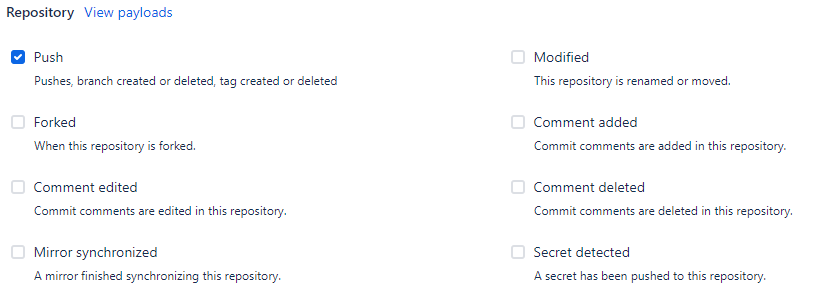
\includegraphics[width=\textwidth]{graphics/bbdc-repository-event-config.png}
    \caption{BitBucket Data Center Webhook Repository Event Config}
    \label{fig:bbdc-repo-event-config}
\end{figure}

\begin{figure}[h]
    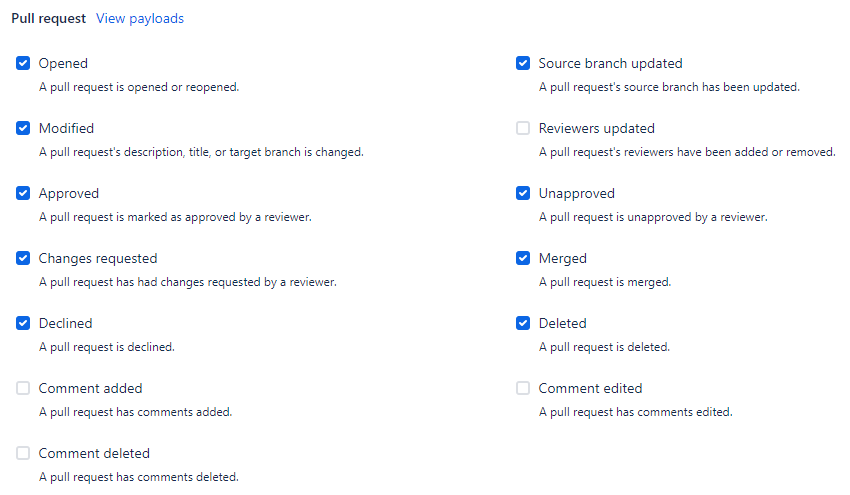
\includegraphics[width=\textwidth]{graphics/bbdc-pr-event-config.png}
    \caption{BitBucket Data Center Webhook Pull Request Event Config}
    \label{fig:bbdc-pr-event-config}
\end{figure}


\section{\cxoneflow HTTP Access Tokens}

While it is possible to use Basic Authorization to access the SCM, typically this is a configuration that
should be avoided.  The Basic Authorization is typically an interactive user account that can be subject
to password changes and Captcha verification that can break \cxoneflow operations.  It is generally
best to use a project-level HTTP Access Token for SCM connection configurations \texttt{api-auth} or
\texttt{clone-auth}.  Please refer to Section \ref{sec:connection-element} for more details about the token
configuration.

Figure \ref{fig:bbdc-token-config} shows the project-level "HTTP Access tokens" configuration.  The required
token permissions for \cxoneflow operations are:

\begin{itemize}
    \item Project read
    \item Repository read\footnote{Figure \ref{fig:bbdc-token-config} shows "Repository write".  There may be future versions of \cxoneflow that will need to create pull-request comments which will require write access.  If desired, the token can be granted "Repository read" until a write capability is released.}
\end{itemize}


\begin{figure}[h]
    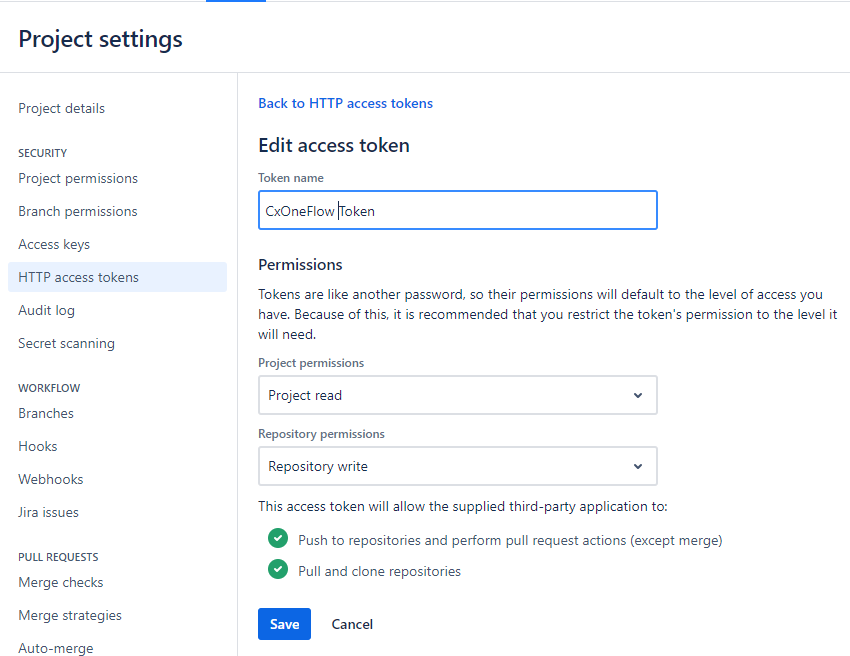
\includegraphics[width=\textwidth]{graphics/bbdc-token-config.png}
    \caption{BitBucket Data Center Project-Level HTTP Access Token Config}
    \label{fig:bbdc-token-config}
\end{figure}

Project-level access tokens do not have an associated user account.  If using project-level
access tokens, one project-level token is required per-project for which \cxoneflow is
orchestrating scans.

\section{\cxoneflow SSH Keys}

While performing scan orchestration, \cxoneflow does access the BitBucket Data Center API for
certain operations.  This requires a configuration in the \texttt{api-auth} configuration
element as described in Section \ref{sec:api-auth-element}.  The \texttt{clone-auth},
described in Section \ref{sec:clone-auth-element}, is an optional element where the credentials
used for cloning code can be provided.  If \texttt{clone-auth} is not provided, cloning will
be attempted using the credentials defined by \texttt{api-auth}.

The \texttt{clone-auth} configuration can define an SSH private key for use in cloning.  This
will allow for a separate set of credentials or authentication methods between cloning and
API use.


\section{Protected Branches}

The \cxoneflow workflow, as described in Section \ref{sec:overview}, uses the concept of "Protected Branches"
to know when to invoke workflows.  BitBucket Data Center allows for the configuration of the branching model
at the project and repository level.  Some repositories inherit their branching model from the project
configuration, but the ability for this to be overridden at the repository level is an optional configuration.
The branching model is used to determine which branches are "Protected Branches".

The project-level branching model configuration is shown in Figure \ref{fig:bbdc-branch-config}.  The
repository-level branching model configuration is similar in that both allow the definition of
"Development" and "Production" branches.  \cxoneflow considers any branch specified as a Development
or Production branch to be a "Protected Branch".

\begin{figure}[h]
    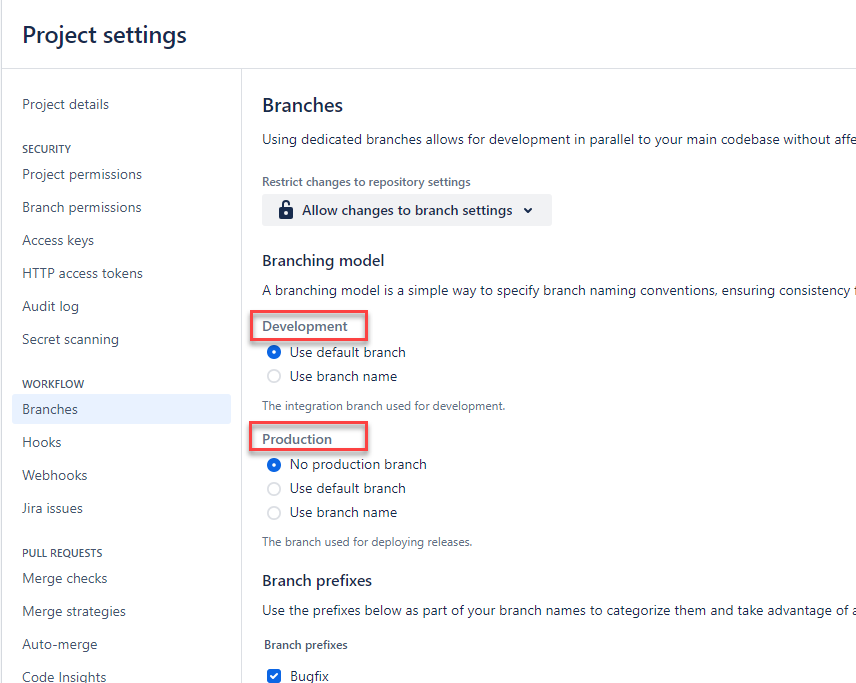
\includegraphics[width=\textwidth]{graphics/bbdc-branch-config.png}
    \caption{BitBucket Data Center Project-Level Branch Config}
    \label{fig:bbdc-branch-config}
\end{figure}




\part{Appendices}
\appendix
\chapter{Release Notes}

\let\sectionold\thesection

\renewcommand\thesection{v}

\section{1.2}

\begin{itemize}
    \item Fixed problem where pooled connections to the SCM would cause PR failures when the network routing 
    fabric discarded the connection route.
    \item BREAKING CHANGE - Added a new configuration option for the CxOneFlow server base URL used to host image
    artifacts used in PR feedback comments.
    \item Fixed an issue with \texttt{ssl-verify} not working with self-signed CAs.
    \item Documentation updates.
\end{itemize}


\section{1.1}

\begin{itemize}
    \item Added more verbose logging to aid in troubleshooting feedback workflows.
    \item Fixed an issue where the feedback scan polling parameters were ignored in some configurations.
    \item Added result summary to PR feedback comments.
    \item If detailed PR feedback comment content exceeds the SCM's comment limit, the comment will be limited to the summary content.
    \item Fixed an issue with the scan permalink published in the PR feedback comments.
\end{itemize}


\section{1.0}

\begin{itemize}
    \item Stabilize Azure DevOps Enterprise Cloud basic authorization implementation.
    \item ADO service hook test ping now fails if the correct shared secret is not provided.
\end{itemize}


\section{0.2 - Beta Release}
   

\begin{itemize}
    \item Support for Azure DevOps Enterprise Cloud.
    \item Pull-request feedback.
\end{itemize}

\section{0.1 - Initial Beta Release}
   

\begin{itemize}
    \item Support for BitBucket Data Center 8.19.2\footnote{Testing was performed against 8.19.2 but it is possible that earlier versions will work.}
    \item Support for Azure DevOps Enterprise 2022.1\footnote{Testing was performed against 2022.1 but it is possible that earlier versions will work.}
    \item Webhook Endpoint support for BitBucket Data Center (BBDC) and Azure DevOps Enterprise (ADOE).
    \item Scan on push to protected branches.
    \item Scan on pull-request targetting protected branches.
    \item Pull-request workflow scan tagging.
\end{itemize}

\let\thesection\sectionold

\chapter{\cxonetext\space Multi-Tenant Endpoint Monikers}
\label{sec:endpoint-monikers}


\section{IAM Endpoint Monikers}

These endpoint monikers correspond to the IAM endpoints referenced in the 
\extlink{https://checkmarx.stoplight.io/docs/checkmarx-one-api-reference-guide/branches/main/ywuqb5n3fas83-authentication-api\#url}{\cxonetext Authentication API} documentation.

\begin{itemize}
    \item US
    \item US2
    \item EU
    \item EU2
    \item DEU
    \item ANZ
    \item India
    \item Singapore
    \item UAE
\end{itemize}


\section{API Endpoint Monikers}

These endpoint monikers correspond to the API endpoints referenced in several
API endpoint descriptions such as the one for 
\extlink{https://checkmarx.stoplight.io/docs/checkmarx-one-api-reference-guide/branches/main/ry3bnvw1ikz2h-projects-rest-api}{\cxonetext Projects REST API} documentation.




\begin{itemize}
    \item US
    \item US2
    \item EU
    \item EU2
    \item DEU
    \item ANZ
    \item India
    \item Singapore
    \item UAE
\end{itemize}

\chapter{\cxoneflowtext\space Developer Information}\label{sec:cxoneflow-development}

The development is performed on Ubuntu using Visual Studio Code.  This is not 
strictly required but any instructions for quick starting the development environment 
will be for using Ubuntu and VSCode. If you have different development tooling you'd like
to use, you'll need to adapt these instructions to fit your tooling.

The target version of Python is currently 3.12.  Using versions prior to 3.12 will likely result in
runtime errors.

\section{Secrets}

\textbf{DO NOT COMMIT SECRETS}

In general, it is a bad idea to commit secrets to the repository.  The \texttt{.gitignore} file is configured
to ignore folders named \texttt{secrets} and YAML files in the root of the code directory.  This 
can be circumvented or other files containing secrets can be inadvertently committed.

If you've committed secrets but not pushed to the public GitHub repository, you can edit the commit history
or merge your clean code into a new clone.  If you've pushed a secret into the public repository, please notify
the other maintainers so the impact can be assessed.

\section{Running with a Debugger}

The VSCode debug menu has a \texttt{Flask} debug task that will run a single endpoint locally.  By default,
the code will attempt to open \texttt{./config.yaml} for the YAML configuration.  Provide a
\texttt{config.yaml} file in the root of your development environment or set the appropriate environment
variables with the path to your \texttt{config.yaml} file.


\section{Installing \LaTeX\space for Documentation}

The documentation is written in LaTeX, so enabling VSCode to lint, compile, and preview
LaTeX requires some configuration.

\subsection{\LaTeX\space Setup}

Follow these steps to install \LaTeX.

\begin{enumerate}
    \item In VSCode, install the "LaTeX Workshop" plugin by James Yu

    \item Install TexLive direct from the website.  This is required since
    most Debian package repositories have an older version of TexLive.
    \begin{enumerate}
        \item Download instructions: \extlink{https://www.tug.org/texlive/acquire-netinstall.html}{https://www.tug.org/texlive/acquire-netinstall.html}
        \item Install instructions: \extlink{https://www.tug.org/texlive/quickinstall.html}{https://www.tug.org/texlive/quickinstall.html}
    \end{enumerate}

    \item At the end of the install, it will instruct you to update `PATH`, `MANPATH`, and `INFOPATH`.
    Set these in `~/.bashrc`, close your shell and re-open it to get the new environment variables.

    \item Execute \texttt{sudo \$(which texconfig) rehash}

\end{enumerate}

If \LaTeX\space is installed correctly, opening any of the \texttt{.tex} files will prove the ability to
compile and preview the manual PDF.



\end{document}
